
\vspace{1cm}

\noindent  \textbf{Leia as instruções antes de fazer a lista:}

\vspace{0.3cm}
\noindent A resolução deve ser entregue em formato Jupyter Notebook ou Google Colab na plataforma Google Classroom, na tarefa designada e até o dia determinado.

\noindent  Não é necessário testar se os dados passados por argumento são válidos a menos que pedido na questão.


\vspace{0.5cm}


\begin{enumerate}[label=\textbf{Q\arabic*.}]


    \item Em um parque de diversões alguns brinquedos só podem ser utilizados por pessoas acima de uma determinada altura. Escreva uma função em Python que recebe por argumento, nesta ordem, uma lista de números inteiros ou floats que representam a altura das pessoas na fila, e um número, que representa a altura mínima necessária para o brinquedo. Sua função deve retornar uma nova lista com a altura somente das pessoas que podem utilizar o brinquedo.

    \item Um sensor ambiental registra leituras de temperatura ao longo do dia em uma lista. Devido a falhas técnicas, algumas leituras registradas são valores negativos inválidos. Escreva uma função em Python que receba por argumento uma lista de temperaturas e remova todas as leituras negativas da própria lista original utilizando o método \code{.pop()}. A função deve retornar o valor médio das temperaturas válidas restantes utilizando \code{sum()} e \code{len()}. Se a lista não contiver nenhuma temperatura válida ao final, retorne \code{0.0}.

    \vspace{0.5cm}
    \item Em uma competição de ginástica artística, a pontuação final de cada atleta é avaliada por um painel de 10 juízes. Para garantir uma avaliação justa, a regra oficial exige descartar apenas uma ocorrência da menor nota e apenas uma ocorrência da maior nota atribuída, somando-se as 8 notas restantes. Escreva uma função em Python que receba por argumento uma lista de números flutuantes (\code{float}) representando as notas de um atleta. A função deve calcular e retornar a soma das notas válidas. A função deve validar o tamanho da entrada, retornando o valor \code{-1} caso a lista contendo as notas não possua exatamente 10 elementos. Em caso de empate nas notas extremas (por exemplo, dois juízes atribuírem a nota mínima), apenas uma dessas notas deve ser descartada. É obrigatório o uso das funções \code{sort()}, \code{sum()} e \code{len()}.
    
    \vspace{0.5cm}
    \item Escreva uma função em Python que recebe duas listas de números inteiros e de mesmo tamanho e retorna uma nova lista na qual, para cada posição, se o elemento daquela posição da primeira lista for igual ao elemento da mesma posição na segunda lista, o valor na lista retornada deve ser 1; se o elemento daquela posição da primeira lista for diferente do elemento da mesma posição da segunda lista, mas este elemento estiver contido na segunda, o valor na lista retornada deve ser 2; se o elemento daquela posição da primeira lista for diferente do elemento da mesma posição da segunda lista e este elemento não estiver contido na segunda, o valor na lista retornada deve ser 0. É permitido o uso das funções \code{range()} e \code{len()} nesta questão. Se as duas listas tiverem tamanhos diferentes, a função deve retornar \code{-1}.

    \vspace{0.5cm}
    \item Escreva uma função em Python que recebe uma lista de listas e retorna o somatório dos produtos dos elementos de cada sublista. Por exemplo, para a entrada \code{([[2,4],[5,2,10]])}, a saída deve ser 108, pois $2 \times 4 + 5 \times 2 \times 10 = 108$. Para essa questão, não utilize a função \code{range()}.


    \item Escreva uma função em Python que receba por argumento uma lista de números (\code{int}ou \code{float}). A função deve verificar a quantidade de elementos da lista e, caso ela esteja vazia ou contenha uma quantidade ímpar de elementos, deve retornar o código de erro \code{-1}. Caso a lista contenha uma quantidade par de elementos, a função deve calcular a média dos valores da lista original, inverter a ordem dos elementos da lista utilizando o método \code{.reverse()} e dividi-la em duas partes iguais. Para entradas válidas, a função deve retornar explicitamente uma saída com 3 valores, nesta exata ordem: \code{media}, \code{lista\_primeira\_metade}, \code{lista\_segunda\_metade}.


    \item (Inspirada na OBI 2023 – Nível 2, Fase 1) Senhor Toupeira é o prefeito de Morro Seco e ao longo dos anos mandou construir muitos túneis embaixo da terra, conectando salões de convivência que ele também mandou construir, para alegria de sua comunidade de toupeiras. Cada túnel conecta exatamente dois salões de convivência distintos e não há dois túneis conectando o mesmo par de salões. Túneis podem ser usados em ambas as direções, ou seja, o túnel que conecta os salões A e B pode ser usado para ir da A para B ou de B para A. Salões de convivência possuem identificadores únicos. Senhor Toupeira agora quer incentivar que as toupeiras de Morro Seco façam caminhadas, para melhorar a saúde da comunidade. Para isso preparou um caderno com várias sugestões de passeio pelos túneis e salões de convivência, em que cada sugestão de passeio é descrita como uma sequência de salões de convivência, que devem ser visitados estritamente na ordem dada. No entanto, Senhor Toupeira foi alertado de que algumas das sugestões de passeio estão incorretas, pois não são possíveis. A figura abaixo mostra um exemplo de salões de convivência e túneis, em que salões têm identificadores 1, 2, 3, 4 e 5.

    \begin{center}
        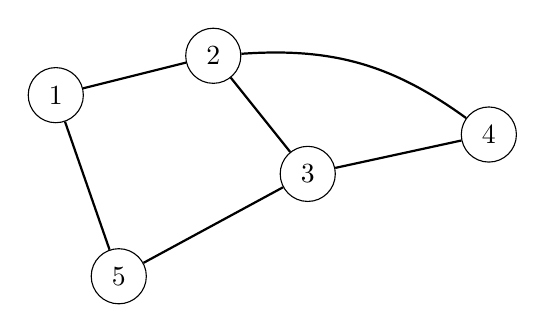
\begin{tikzpicture}[node distance=1.8cm, auto, every node/.style={circle, draw, minimum size=0.7cm, inner sep=0pt}]
            % Nós
            \node (1) at (0, 1.5) {1};
            \node (2) at (2, 2) {2};
            \node (3) at (3.2, 0.5) {3};
            \node (4) at (5.5, 1) {4};
            \node (5) at (0.8, -0.8) {5};

            % Arestas
            \draw[thick] (1) -- (2);
            \draw[thick] (1) -- (5);
            \draw[thick] (2) -- (3);
            \draw[thick] (2) to[bend left=20] (4);
            \draw[thick] (3) -- (4);
            \draw[thick] (3) -- (5);
        \end{tikzpicture}
    \end{center}

    Um passeio composto pela sequência de salões \{5, 3, 4, 3, 2\} é possível. Mas o passeio composto pela sequência de salões \{2, 3, 5, 4\} não é possível, pois não existe túnel entre os salões 5 e 4. Sua tarefa é escrever uma função em Python que recebe por argumento uma lista de listas que indica as conexões entre os salões e outra lista de listas com possíveis passeios, e retorna um número inteiro que informa a quantidade de passeios que são possíveis. O primeiro argumento é uma lista de listas onde cada sublista contém somente dois elementos que indicam as conexões entre dois salões. Por exemplo, a figura acima pode ser representada por \code{[[1, 2], [1, 5], [2, 3], [3, 5], [2, 4], [4, 3]]}, mas a ordem dos números é indiferente, de forma que as listas de listas \code{[[2, 1], [5, 1], [3, 2], [3, 5], [4, 2], [4, 3]]} e \code{[[2, 3], [3, 4], [4, 2], [3, 5], [1, 5], [1, 2]]} também representam as conexões dessa mesma figura. O segundo argumento é uma lista de listas onde cada sublista representa um possível passeio. Por exemplo, a lista \code{[[5, 3, 4, 3, 2], [2, 3, 5, 4]]} indica dois possíveis passeios (que são os passeios do exemplo acima). Para essas entradas, a saída deveria ser 1, pois somente um dos dois passeios indicados é possível.

    
\end{enumerate}